\chapter{Discovery and The Manufacture of Soft Drinks}\label{ch3}

\subsection{Some History of Soft Drinks}
The consumption of soft drinks has taken form for many centuries and was initially first used in fermented barley drinks that contained herbs and alcohol to kill any diseases or bacteria in the water, making it safe to drink. As time went on, the first officially marketed soft drink was a drink containing lemon juice with honey (Steen and Ashurst, 2006). Of course at this time the only way to get carbon dioxide within a drink was fermentation of beers and wines; moreover, the push to study carbonated drinks was pushed forward as the natural springs and spas in Holland \& Pyrmont and Seltzer in Germany were known for their therapeutic use. Though the claims for the therapeutic and medicinal properties of carbonated drinks were largely exaggerated, they still had a ‘fizz’ that made the drink more palatable and visually appealing. \\

As the soft drink industry grew, there were more than 50 manufacturers in the 1840’s just in London. Popular carbonated beverage company J.Schweppe \& Co. had paid £5000 for the licence to sell soda and mineral waters at this time, equating to roughly \$355,000 AUD today. \\

\subsection{Discovery of Carbon Dioxide}
Carbon dioxide was one of the first studied gases that was seen as different from regular air. Belgian scientist Jan Baptista van Helmont was one of the first to note the effects of carbon dioxide when he burned charcoal in a closed vessel and noted the difference of mass in the ash and charcoal before. He hypothesised that the rest of the charcoal had transformed into an invisible substance that he named ‘gas silvestre’ (carbon dioxide) (Chastain, 2019). \\
Later, Scottish scientist Joseph Black found that when limestone (calcium carbonate) was heated, it would form a gas he called ‘fixed air’. \newpage It was observed that this gas was denser than normal air; we now know that carbon dioxide has a density of \begin{math}1.98 kg/m^3\end{math} at standard conditions. roughly ~1.5 times more dense than air (Univerzita Karlova, 2023), and that this gas could not support animal or plant life (Robert G.W. Anderson, 2019). It was also discovered that when this was bubbled in an aqueous solution of calcium hydroxide (lime), it would form calcium carbonate, making the solution milky, as shown in Fig 3.1 (Smith and Davis, 2017). \\

\begin{figure}[htp]
    \centering
    \[
        Ca(OH)_{2} \ + \ CO_{2} \to CaCO_{3} + H_{2}O \\
        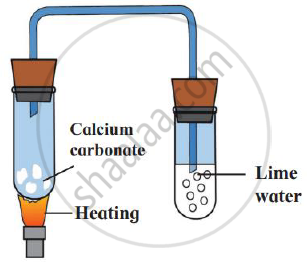
\includegraphics[width=0.5\linewidth]{assets/4.png}
    \]
    \caption{Chemical reaction of lime water and carbon dioxide gas forming calcium carbonate participate.}
    \label{fig:enter-label}
\end{figure}

\subsection{Water Treatment}
Firstly, in the production line of soft drinks, water is sourced, and this water (in Europe) must meet a standard with the EC Drinking Water Directive 80/778/EEC, and if this water is not up to standard, there may be acute or adverse effects over a short or long period of time. Contamination may include, but is not limited to, heavy metal poising, chemical irritant exposure, \& biological hazards such as E. coli or cholera (Directive (EU), 2020).\\
Firstly, the water is passed through tanks that contain sand, filtered gravel, and coarse gravel; this process ensures that the water is free of any foreign mass or organic matter. \newpage
A common method to disinfect the water of any organisms is by using chlorine and sodium hypochlorite; in this process, 6–8 mg/L of chlorine is added to sterilise the water. At this amount, chlorine will oxidise all impurities, removing taste and odour caused by phenol (used to make plastics, explosives, and drugs such as aspirin) or other similar substances (Wade, 2018) (Griffiths, 2016).
When dissolving chlorine in water, it forms hydrochloric acid and hypochlorous acids. \newline
\begin{center}
    \begin{math}
    Cl_{2} + H_{2}O = HCl + HOCl
\end{math}
\end{center}

Due to hypochlorous acid being a weak acid, it dissociates, giving off a hypochlorite ion.

\begin{center}
    \begin{math}
    HOCl = H^{2} + OCl^{-} 
\end{math}
\end{center}


After this process, the sterilised water is then passed through a series of carbon filters, which work to de-chlorinate the solution.
\begin{figure}[htp]
    \centering
    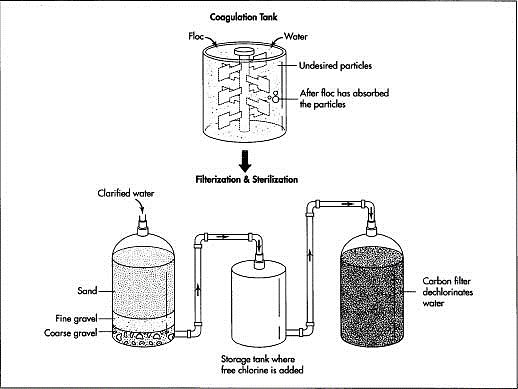
\includegraphics[width=0.5\linewidth]{assets/5.png}
    \caption{Water filter and sterilisation within a manufacturing plant.}
    \label{fig:enter-label}
\end{figure}

\section{Carbonation}
When carbon dioxide is dissolved in water (Fig 3.3 \& 3.4), the solubility of \begin{math}CO_{2}\end{math} varies depending on the surrounding pressure, so when water is carbonated, it is typically kept at 2.04–2.38 atm (30–35 psi) as this makes it so the water is able to dissolve more gas easily (Camp Keg, 2024). The solubility is affected negatively by higher temperatures and is affected positively at higher pressures, at \begin{math}15.5^O C \end{math}and at a pressure of 1 atm. The main purpose of this process is to form carbonic acid (\begin{math}H_{2}CO_{3}\end{math}), which partly dissociates to form bicarbonate and carbonate ions (Steen and Ashurst, 2006). \\

\begin{figure}[htp]
    \centering
    \[
        CO_{2}(g) + H_{2}O(l) \rightleftharpoons H_{2}CO_{3}
    \]
    \caption{Carbon dioxide being dissolved into water forming carbonic acid.}
    \label{fig:enter-label}
\end{figure}

\begin{figure}[htp]
    \centering
    \[
        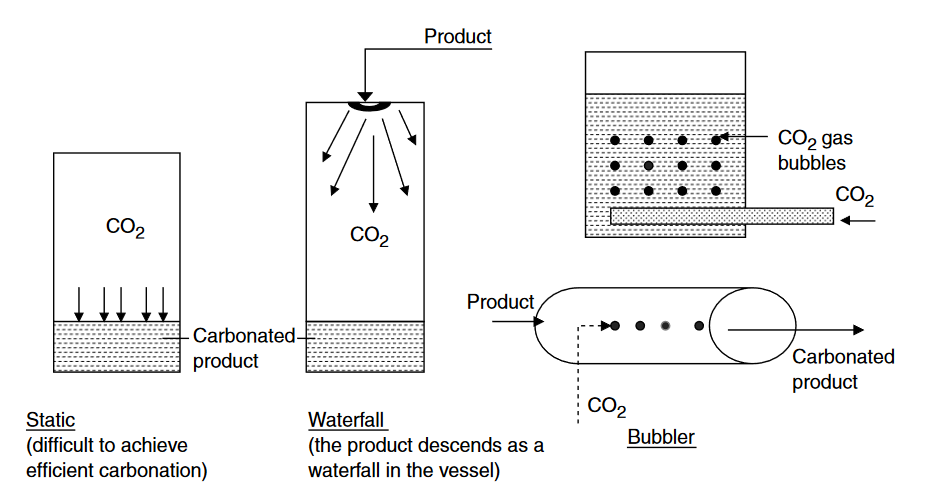
\includegraphics[width=0.5\linewidth]{assets/6.png}
    \]
    \caption{Typical carbonation system (Steen and Ashurst, 2006, p 130).}
    \label{fig:enter-label}
\end{figure}

\newpage

When carbonic acid is formed, it is a diprotic acid that has two hydrogen's that can disassociate into two salts, either hydrogen carbonates (\begin{math}HCO_{3} ^-\end{math} )  or carbonates on their own (\begin{math}CO_{3} ^2-\end{math}) (Britannica, 2019).

\begin{figure}[htp]
    \centering
    \[
        H_{2}CO3 + H_{2}O \rightleftharpoons H_{3}O^+ + HCO_{3}^{\ -} \\
        K_{a1} = 2.5 * 10^{-4} mol/L \ ; \ _{p}K_{a1} = 3.60 \ at \ 25 °C.
    \]
\end{figure}
          

The formation of hydrogen ions decreases the pH within the system and makes the overall product acidic.

The standard machinery used for this is the simple in-line carbonator (Fig X), which injects gas bubbles into the liquid in a stream. This process allows more formation of gas bubbles due to the high surface area, leading to more dissolved carbon dioxide gas into the mixture.

\begin{figure}[htp]
    \centering
    \[
        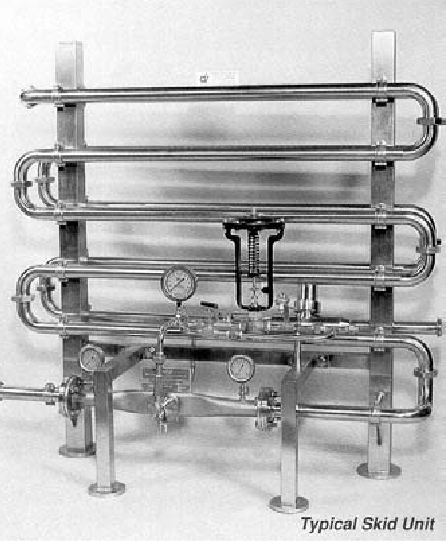
\includegraphics[width=0.5\linewidth]{assets/7.png}
    \]
    \caption{Simple in-line carbonator (Canongate Technology).}
    \label{fig:enter-label}
\end{figure}

\newpage

\section{PET Bottling}
When the water is incorporated with the sugar syrup and is carbonated, it needs to go into a container; this is where polyethylene terephthalate (PET) comes in.
PET is a polyester polymer that is made up of alternating ethylene glycol and terephthalic acid molecules. PET was first used as a fibre for textiles in the 1940’s and is still used for many clothing products. You may recognise PET from its generic name, polyester. PET was first used for soft drinks in the 1970's, as it made the production costs of drinks much cheaper when compared to glass bottles (Syrett, 2006).

To produce satisfactory PET pellets, the reaction occurs within an esterification reactor; this is the process of combining an organic acid, such as terephthalic acid used in this reaction, with an alcohol, such as ethylene glycol, which gives out an ester molecule (BYJU'S, 2022).

\begin{figure}[htp]
    \centering
    \[
        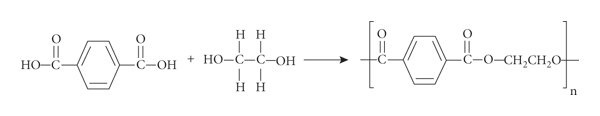
\includegraphics[width=0.5\linewidth]{assets/9.png}
    \]
    \caption{The polymerisation reaction of terephthalic acid and ethylene glycol. (Wiley Journal of Chemistry, 2020)}
    \label{fig:enter-label}
\end{figure}
\begin{figure}[htp]
    \centering
    \[
        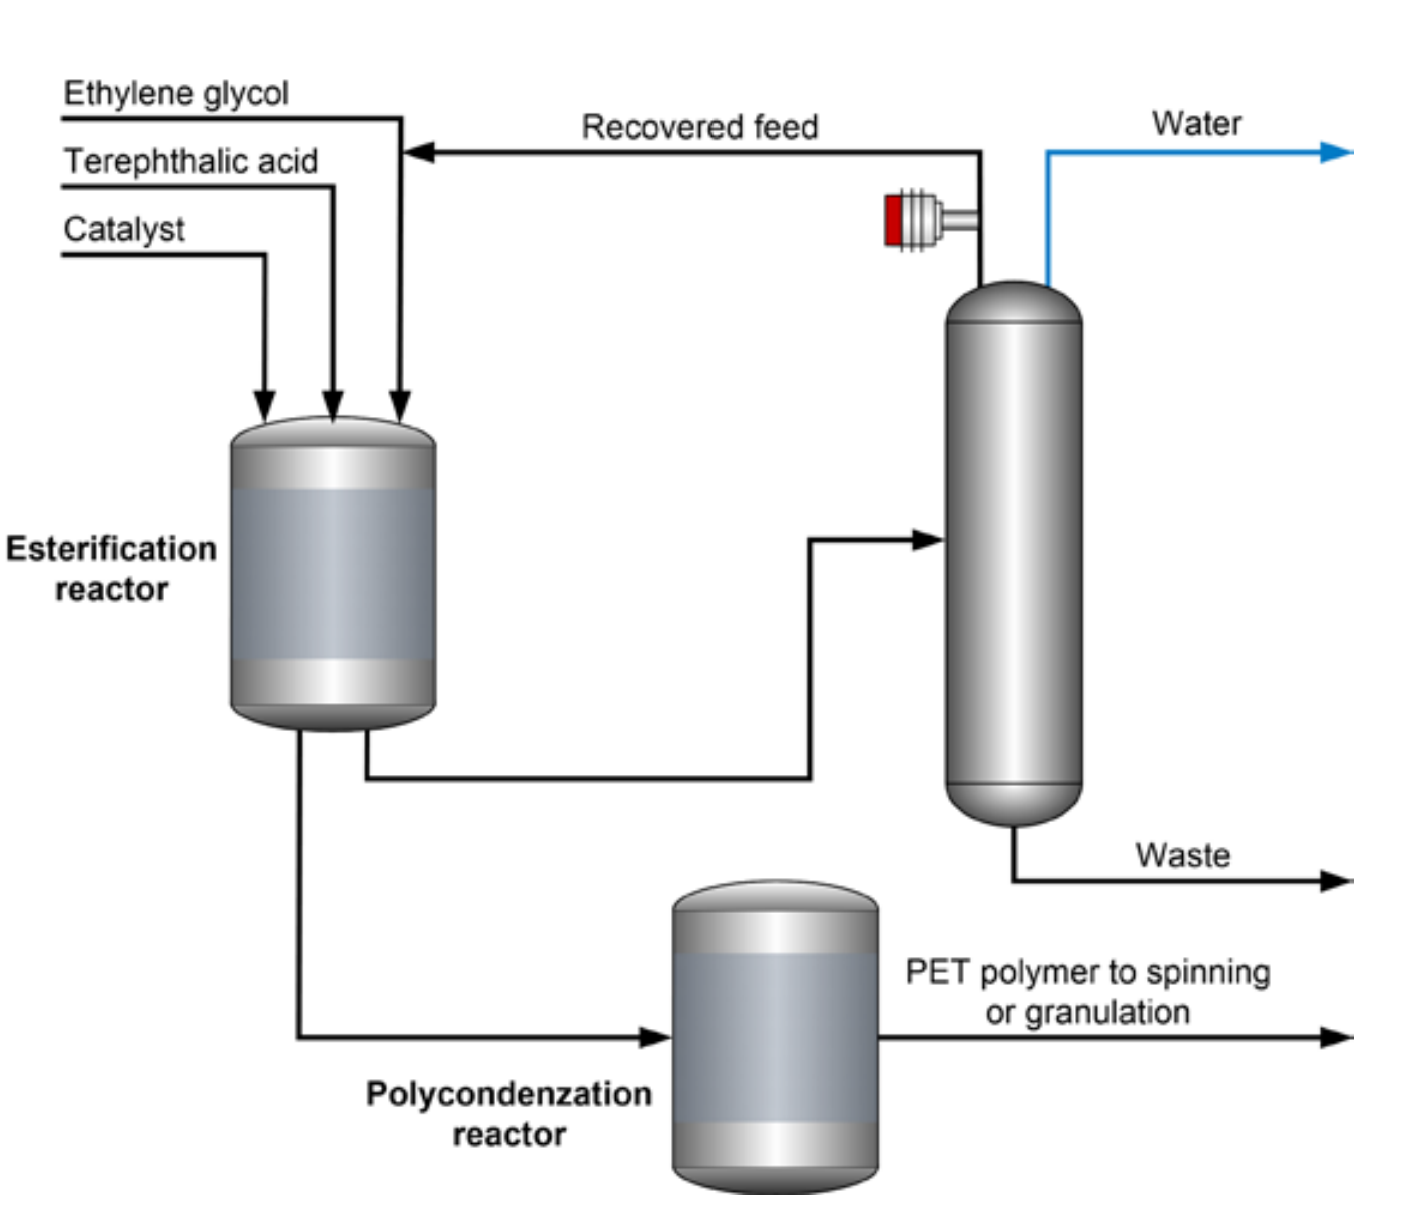
\includegraphics[width=0.5\linewidth]{assets/10.png}
    \]
    \caption{Polyethylene terephthalate (PET) production process. (Vaisala, 2023)}
    \label{fig:enter-label}
\end{figure}
\newpage

After this process, PET pellets are used in injection moulding to create plastic bottles. Firstly, the pellets are melted at \begin{math}240 to 280^{O}C\end{math}, and colours are added at this time if needed. Following this, compressed air is blown into the moulds at 80 to 140 MPa to shape the plastic into the mould to produce a bottle. At this stage, though, the plastic is still at a high temperature and needs to be cooled in a water bath due to the fast cooling process, vital for shorter production time (WKAI, 2024).  

\begin{figure}[htp]
    \centering
    \[
        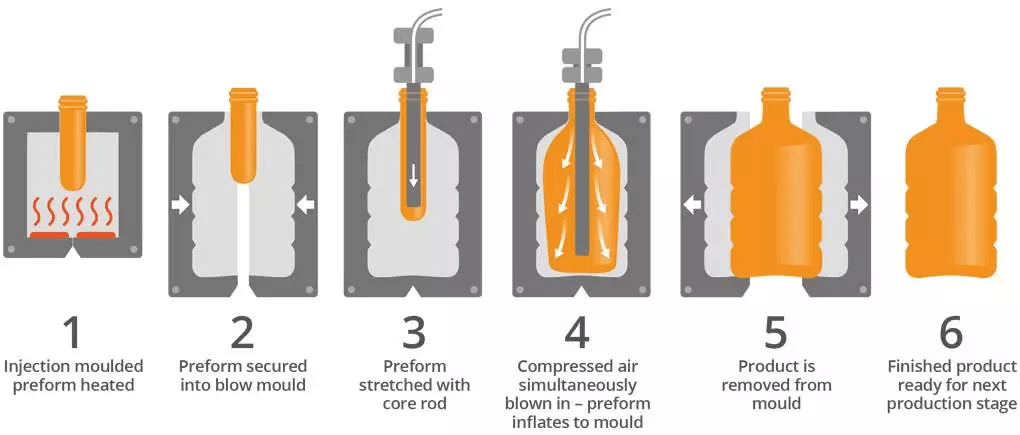
\includegraphics[width=0.5\linewidth]{assets/11.png}
    \]
    \caption{Injection stretch blow moulding process (Robinson Packaging, 2023)}
    \label{fig:enter-label}
\end{figure}

\section{A Solution To Cap Loss}
After this beautiful process of bottles filling up, they need a lid to close them, so another round of PET injection moulding occurs where a PET screw-design cap is made. Austrian company ALPLA WERKE ALWIN LEHNER GMBH \& CO. KG had designed a closure cap that contained a threaded inner neck with a threaded counter closure cap that included a tamper-proof ring. This invention meant that the bottle could not be opened without breaking the tamper-proof ring. \newpage This adds a layer of protection not only to the consumer but also to the manufacturer, as any liability could be passed onto the supplier. Additionally, the tamper-proof ring also included a plastic tab joining it to the base of the closing cap.   addition is due to new EU regulations about plastic waste reduction due to litter, as many plastic caps are thrown into the natural environment or disposed of improperly (ALPLA WERKE ALWIN LEHNER GMBH \& CO. KG and RIEDERER HASLER \& PARTNER PATENTANWÄLTE, 2022).

\begin{figure}[htp]
    \centering
    \[
        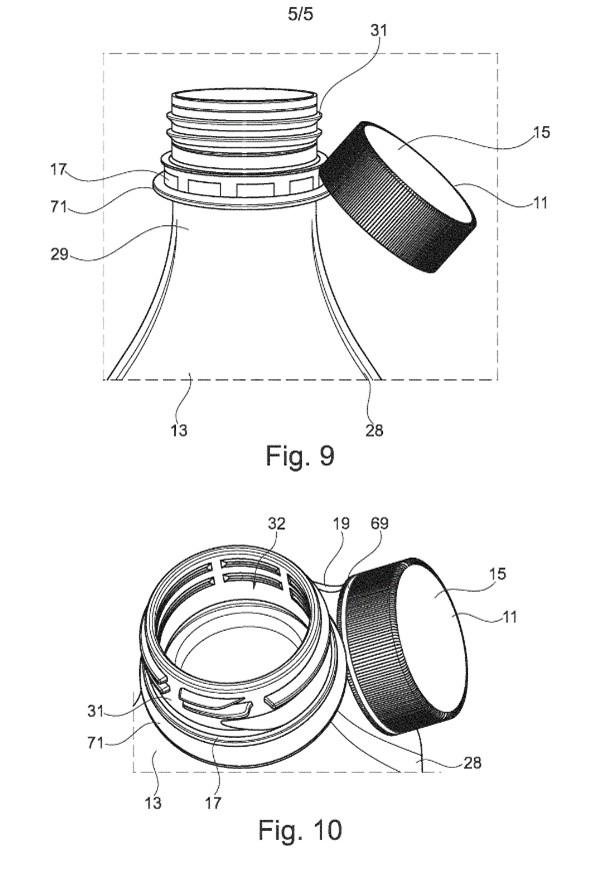
\includegraphics[width=0.5\linewidth]{assets/12.png}
    \]
    \caption{Claimed solution in the patent (ALPLA WERKE ALWIN LEHNER GMBH \& CO. KG, 2022).}
    \label{fig:enter-label}
\end{figure}

\section{Labelling}
Following the closure process, labels are applied to the product to distinguish it from other competing products. Two industry standard methods are used: patch labelling and wraparound labelling. In patch labelling, a system of sponges, glue rollers, and brushes is used to smooth a precut label and then apply it to the bottle, using a rotary machine to achieve clamping of the bottles at all times.
\newpage
\begin{figure}[htp]
    \centering
    \[
        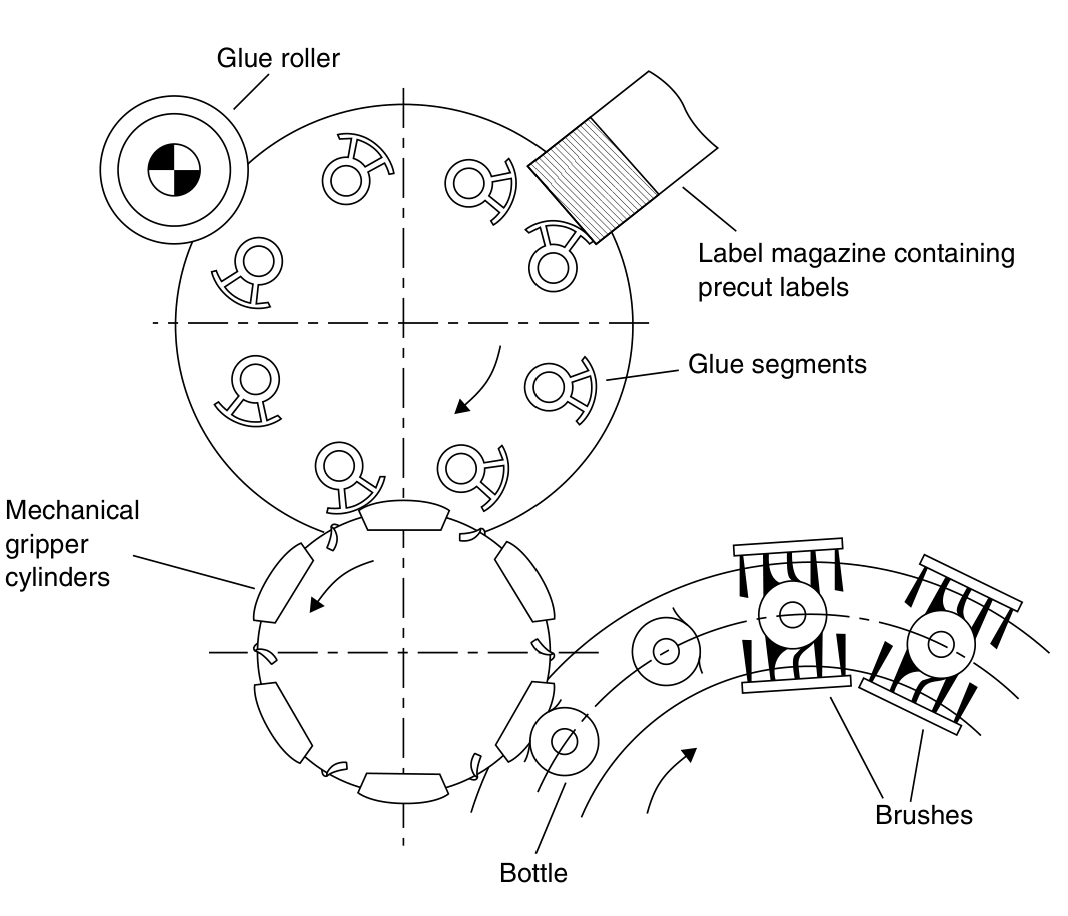
\includegraphics[width=0.5\linewidth]{assets/13.png}
    \]
    \caption{Patch Labelling (Krones UK Ltd).}
    \label{fig:enter-label}
\end{figure}

In wraparound labelling a magazine containing the labels, the first glue station applies a rough coat to the bottles to prepare them to have their labels applied to them; in the second glue station, a very narrow amount of glue is applied to pull the label from the magazine, and then brushes are used to smooth the label around the bottle; this process can be seen in Figure 3.11.

\begin{figure}[htp]
    \centering
    \[
        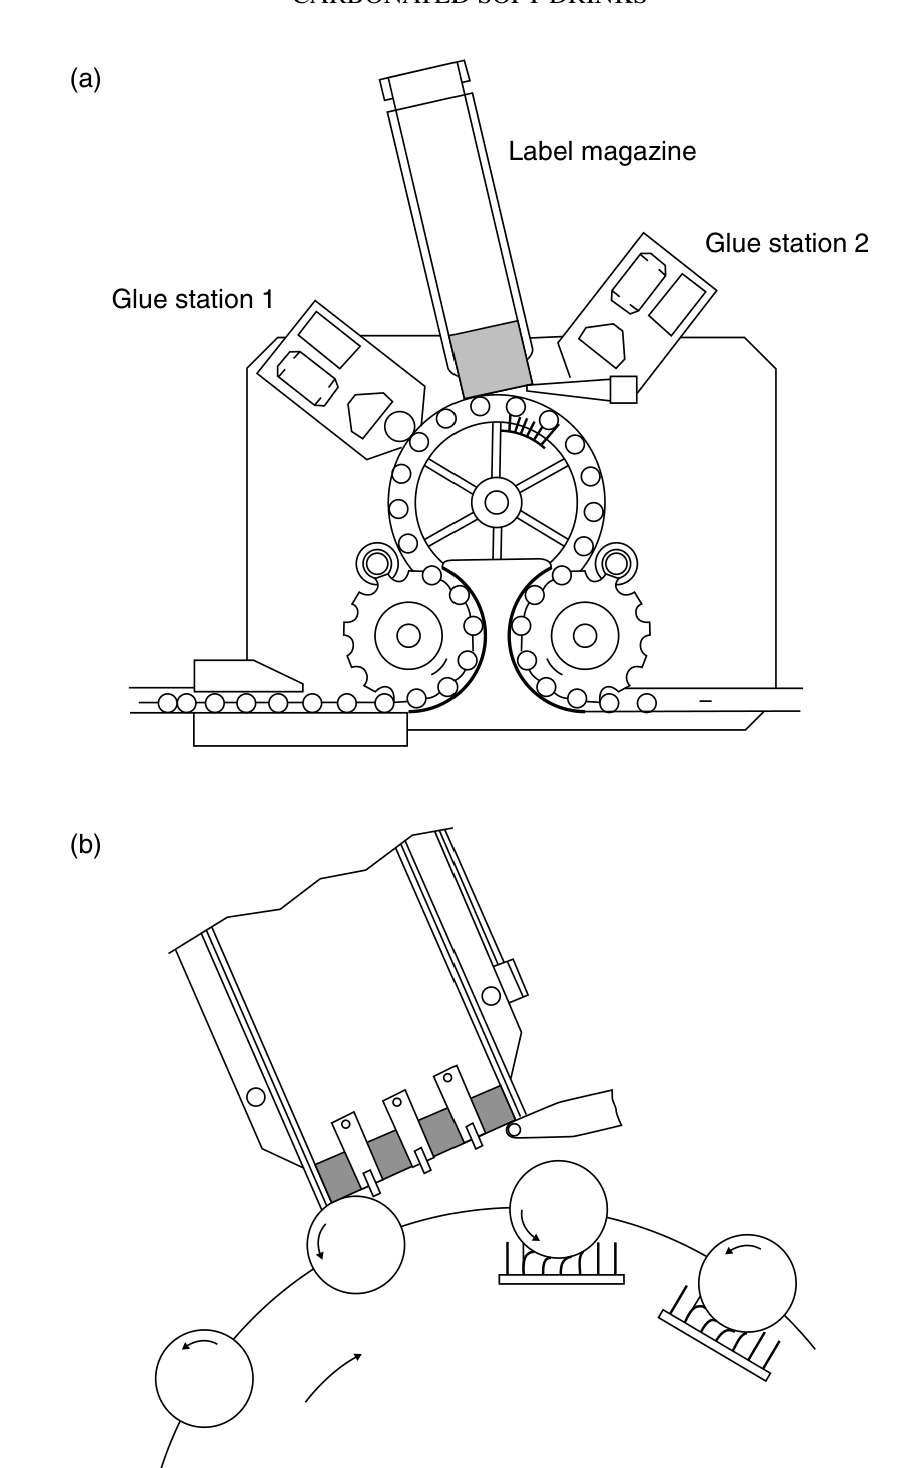
\includegraphics[width=0.5\linewidth]{assets/14.png}
    \]
    \caption{Wraparound Labelling (Krones UK Ltd).}
    \label{fig:enter-label}
\end{figure}


\newpage
\section{But Why These Condition's?}
Using this knowledge about the system of carbon dioxide dissolving into water to form carbonic acid, as stated in figure X, we can use collision theory to estimate why this reaction happens. For the carbon dioxide molecules to form anything, they need a sufficient amount of energy to collide with the water molecules to form carbonic acid, and chapter \ref{ch02} states that these collisions are affected by external conditions. In this system, pressure and temperature are very important factors due to carbonic acid being unstable and spontaneous due to its Gibbs free energy calculation seen below at standard conditions (Bross, 2011) : \\
\begin{figure}[htp]
    \centering
    \[
        \Delta G^{o}_{f} (H_{2}CO_{3}) \cong -612.96 \ kJ / mol
    \]
    \caption{Gibbs free energy for carbonic acid (Bross, 2011).}
    \label{fig:enter-label}
\end{figure}
\newpage

Firstly, when the temperature is higher in the system, there is more kinetic energy for both the \begin{math}CO_{2}\end{math} and \begin{math}H_{2}O\end{math} molecules to collide with each other. You may think that this would lead to more carbonic acid being formed but this theory is mistaken, This may increase the reaction rate but it will not form carbonic acid due to the dissolved carbon dioxide having too much energy, it will favour the reverse reaction and turn back into its gaseous state. This is what happens when you leave a soda can out in the sun for too long and try to drink it; it may seem ‘flat’ or not fizzy anymore. This is why manufacturers recommend the carbonated drinks be stored at low temperatures and away from direct sunlight, as it reduces the amount of collisions, slowing down the release of carbon dioxide.

Secondly, pressure also plays a role in this system with the concentration of carbon dioxide within the drink. When there is a higher force of pressure within the system, this forces both the carbon dioxide and water molecules to collide more, leading to more carbonic acid to form. This is due to Le Chateliers principle, also described in Chapter \ref{ch02}. In the reaction, there is one molecule of carbon dioxide and one molecule of water both on the left side, while there is only one molecule of carbonic acid on the right side of the reaction. This shift of pressure means the equation will shift to the side of fewer molecules when the reaction takes place. 
This is why the water is injected with a high-pressure stream of carbon dioxide during the carbonation process and then subsequently kept at a high pressure when bottling the product to keep the reaction at equilibrium, but upon opening the bottle the equilibrium gets shifted to the left side and the reaction favours the decomposition of carbonic acid back to its carbon dioxide and water counterparts.
\begin{figure}[htp]
    \centering
    \[
        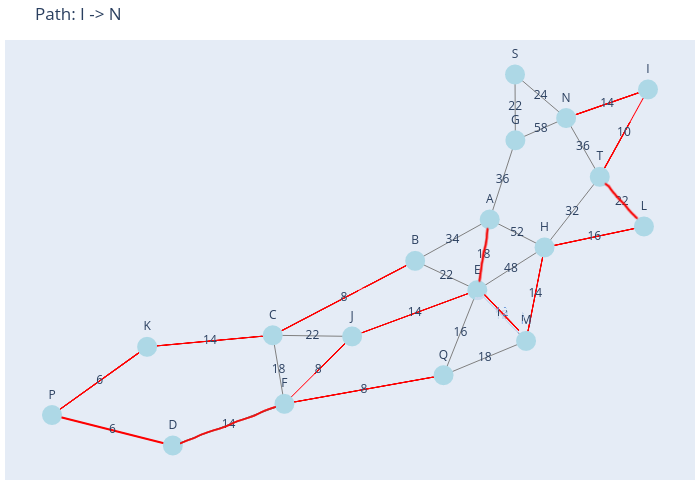
\includegraphics[width=0.5\linewidth]{assets/15.png}
    \]
    \caption{Molecular diagram showing the amount of moles per side of reaction (ACS, 2023).}
    \label{fig:enter-label}
\end{figure}

As seen in both factors, the high pressure of carbon dioxide not only provides more collisions with the water molecules to form carbonic acid, but it also makes the solution more soluble, favouring dissolution, in addition to the low temperature that then reduces the kinetic energy within the molecules, which favours the formation of carbonic acid.
